\newif\ifshowsolutions
\showsolutionstrue
\documentclass{article}
\usepackage{listings}
\usepackage{amsmath}
%\usepackage{subfigure}
\usepackage{subfig}
\usepackage{amsthm}
\usepackage{amsmath}
\usepackage{amssymb}
\usepackage{graphicx}
\usepackage{mdwlist}
\usepackage[colorlinks=true]{hyperref}
\usepackage{geometry}
\usepackage{titlesec}
\geometry{margin=1in}
\geometry{headheight=2in}
\geometry{top=2in}
\usepackage{palatino}
\usepackage{mathrsfs}
\usepackage{fancyhdr}
\usepackage{paralist}
\usepackage{todonotes}
\setlength{\marginparwidth}{1.15cm}
\usepackage{tikz}
\usetikzlibrary{positioning,shapes,backgrounds}
\usepackage{float} % Place figures where you ACTUALLY want it
\usepackage{comment} % a hack to toggle sections
\usepackage{ifthen}
\usepackage{mdframed}
\usepackage{verbatim}
\usepackage[strings]{underscore}
\usepackage{listings}
\usepackage{bbm}
\def\eps{\varepsilon}
\rhead{}
\lhead{}

\renewcommand{\baselinestretch}{1.15}

% Shortcuts for commonly used operators
\newcommand{\E}{\mathbb{E}}
\newcommand{\Var}{\operatorname{Var}}
\newcommand{\Cov}{\operatorname{Cov}}
\newcommand{\Bias}{\operatorname{Bias}}
\newcommand{\R}{\mathbb{R}}
\newcommand{\E}{\mathbb{E}}
\newcommand{\ds}{\displaystyle}
\DeclareMathOperator{\argmin}{arg\,min}
\DeclareMathOperator{\argmax}{arg\,max}

% do not number subsection and below
\setcounter{secnumdepth}{1}

% custom format subsection
\titleformat*{\subsection}{\large\bfseries}

% set up the \question shortcut
\newcounter{question}[section]
\newenvironment{question}[1][]
  {\refstepcounter{question}\par\addvspace{1em}\textbf{Question~\Alph{question}\!
    \ifthenelse{\equal{#1}{}}{}{ [#1 points]}: }}
    {\par\vspace{\baselineskip}}

\newcounter{subquestion}[question]
\newenvironment{subquestion}[1][]
  {\refstepcounter{subquestion}\par\medskip\textbf{\roman{subquestion}.\!
    \ifthenelse{\equal{#1}{}}{}{ [#1 points]:}} }
  {\par\addvspace{\baselineskip}}

\titlespacing\section{0pt}{12pt plus 2pt minus 2pt}{0pt plus 2pt minus 2pt}
\titlespacing\subsection{0pt}{12pt plus 4pt minus 2pt}{0pt plus 2pt minus 2pt}
\titlespacing\subsubsection{0pt}{12pt plus 4pt minus 2pt}{0pt plus 2pt minus 2pt}


\newenvironment{hint}[1][]
  {\begin{em}\textbf{Hint: }}{\end{em}}

\ifshowsolutions
  \newenvironment{solution}[1][]
    {\par\medskip \begin{mdframed}\textbf{Solution~\Alph{question}#1:} \begin{em}}
    {\end{em}\medskip\end{mdframed}\medskip}
  \newenvironment{subsolution}[1][]
    {\par\medskip \begin{mdframed}\textbf{Solution~\Alph{question}#1.\roman{subquestion}:} \begin{em}}
    {\end{em}\medskip\end{mdframed}\medskip}
\else
  \excludecomment{solution}
  \excludecomment{subsolution}
\fi




%%%%%%%%%%%%%%%%%%%%%%%%%%%%%%
% HEADER
%%%%%%%%%%%%%%%%%%%%%%%%%%%%%%

\chead{%
  {\vbox{%
      \vspace{2mm}
      \large
      Machine Learning \& Data Mining \hfill
      Caltech CS/CNS/EE 155 \hfill \\[1pt]
      Homework 6, 26 tokens used, Jagath Vytheeswaran\hfill
      February 2019 \\
    }
  }
}

\begin{document}
\pagestyle{fancy}

%%%%%%%%%%%%%%%%%%%%%%%%%%%%%%
% POLICIES
%%%%%%%%%%%%%%%%%%%%%%%%%%%%%%

\section{Class-Conditional Densities for Binary Data [25 Points]}

\problem[5] Parameters of Full Model with Factorizing
\begin{subsolution}
\begin{figure}[H]
	\centering
	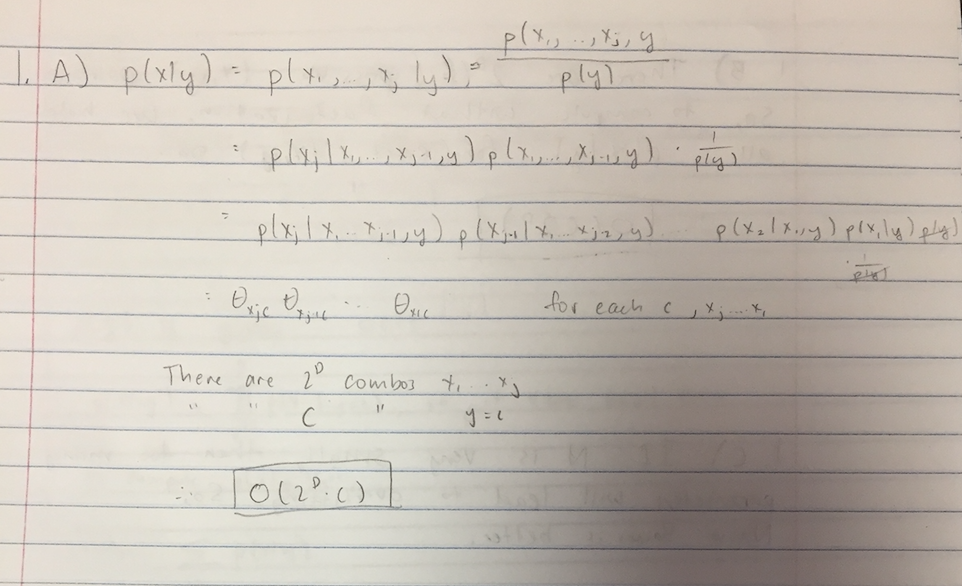
\includegraphics[width=0.95\textwidth]{img/set6template-58a4d205.png}
	\caption{}
	\label{}
\end{figure}
\end{subsolution}
\clearpage

\problem[5] Parameters of Full Model without Factorizing
\begin{subsolution}
\begin{figure}[H]
	\centering
	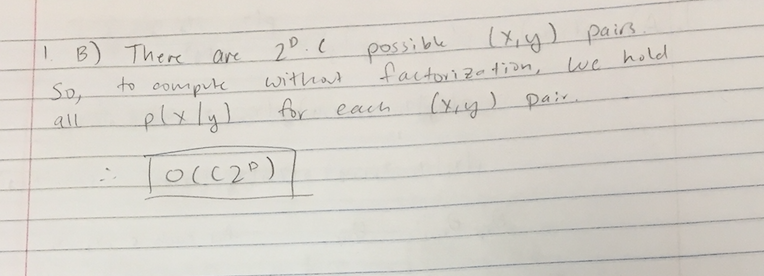
\includegraphics[width=0.95\textwidth]{img/set6template-ee5d9c5d.png}
	\caption{}
	\label{}
\end{figure}
\end{subsolution}
\clearpage

\problem[2] Naive Bayes vs. Full Model for Small $N$
\begin{subsolution}
\begin{figure}[H]
	\centering
	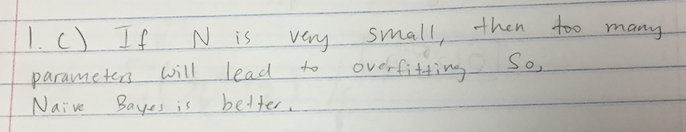
\includegraphics[width=0.95\textwidth]{img/set6template-2bc0bc78.png}
	\caption{}
	\label{}
\end{figure}
\end{subsolution}
\clearpage

\problem[2] Naive Bayes vs. Full Model for Large $N$
\begin{subsolution}
\begin{figure}[H]
	\centering
	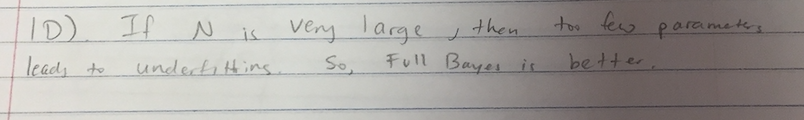
\includegraphics[width=0.95\textwidth]{img/set6template-fae955f2.png}
	\caption{}
	\label{}
\end{figure}
\end{subsolution}
\clearpage

\problem[11] Computational Complexity of Making a Prediction Using Naive Bayes vs Full Model
\begin{subsolution}
\begin{figure}[H]
	\centering
	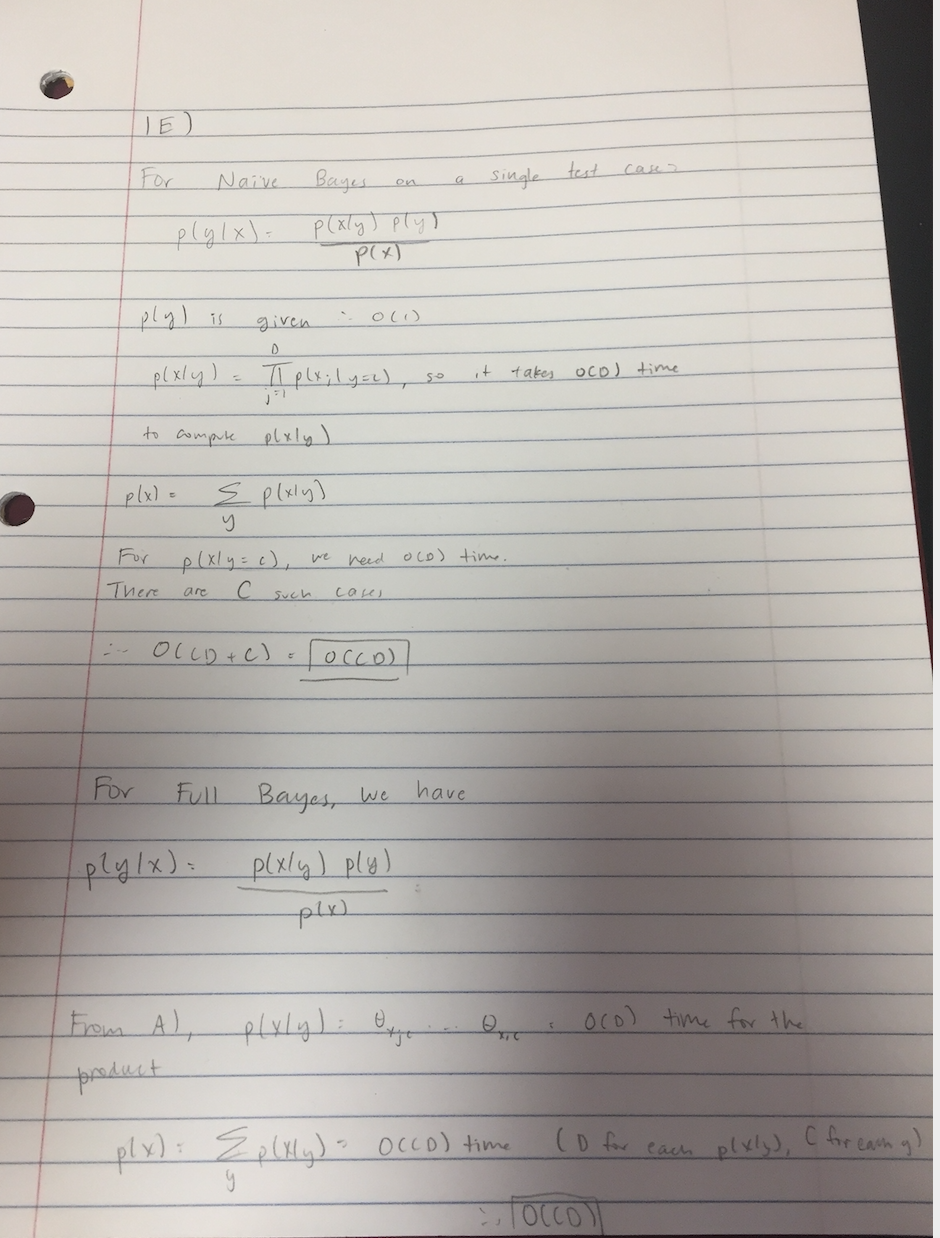
\includegraphics[width=0.65\textwidth]{img/set6template-1d71be37.png}
	\caption{}
	\label{}
\end{figure}
\end{subsolution}
\clearpage


\newpage
\section{Sequence Prediction [75 Points]}

\indent\problem[10] % indent for consistency
Max-Probability State Sequences for 6 Trained HMMs
\begin{subsolution}
  \begin{figure}[H]
  	\centering
  	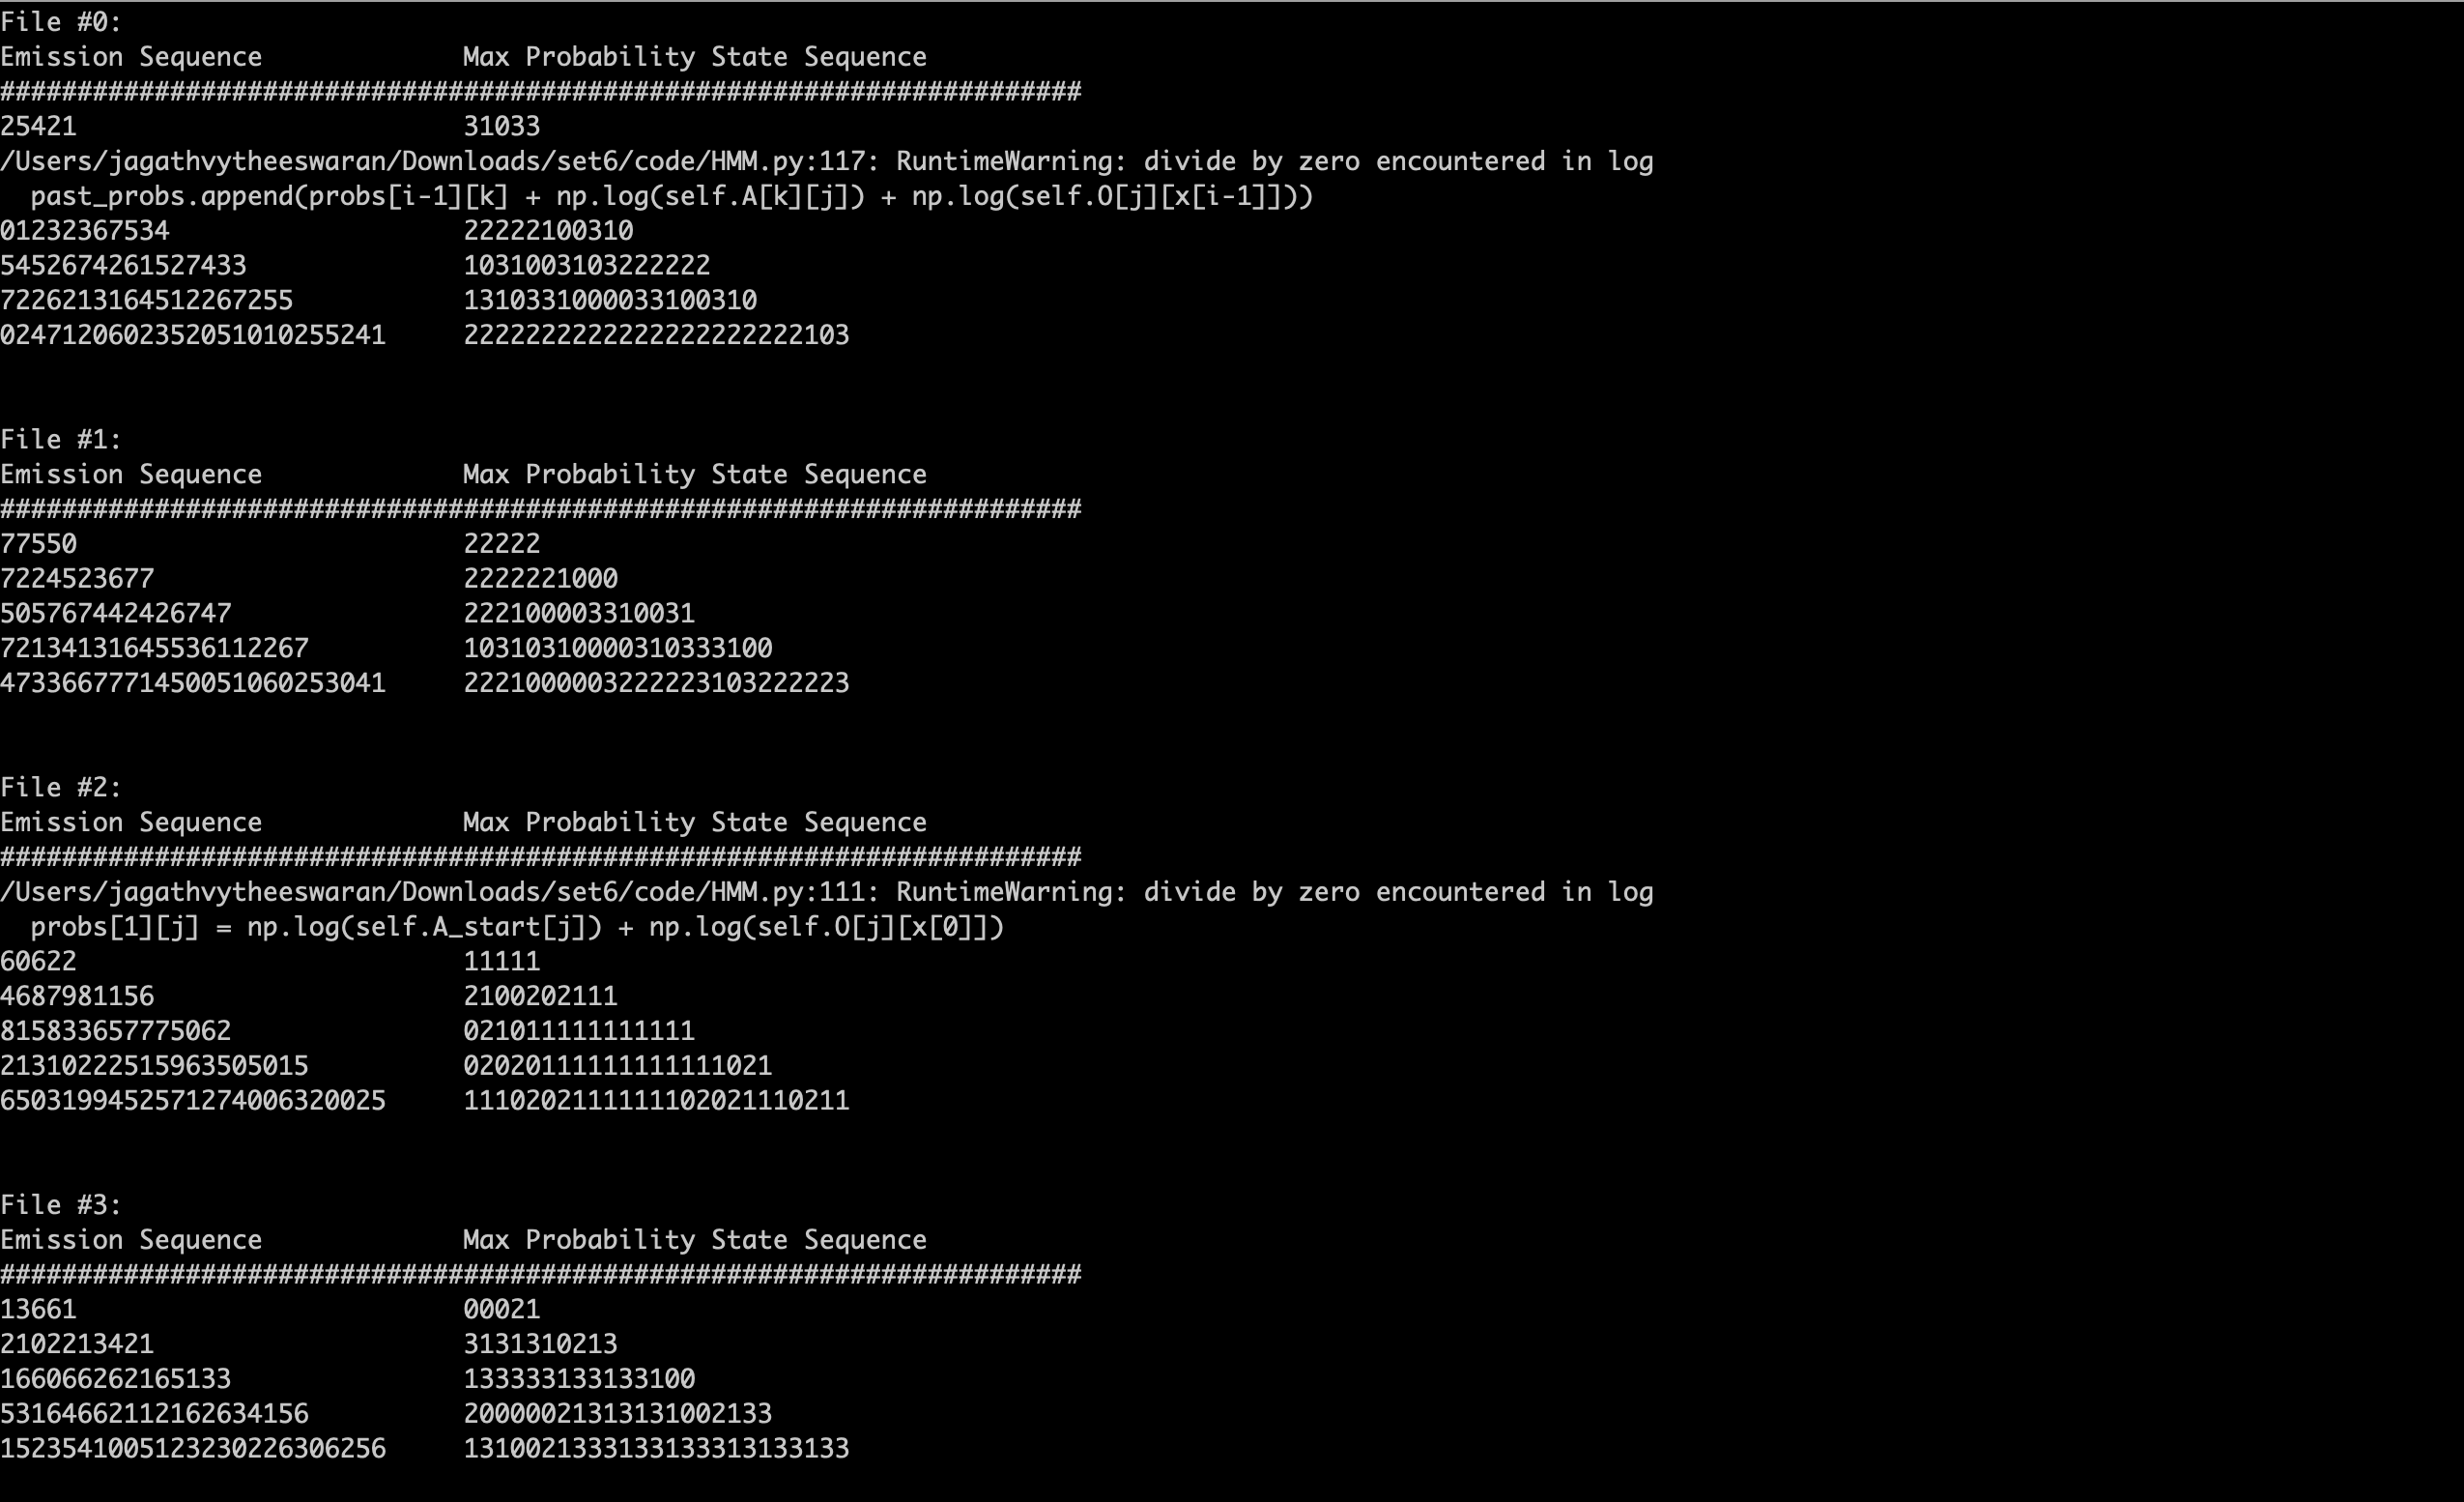
\includegraphics[width=0.5\textwidth]{img/set6template-7edca5b3.png}
  	\caption{}
  	\label{}
  \end{figure}

  \begin{figure}[H]
  	\centering
  	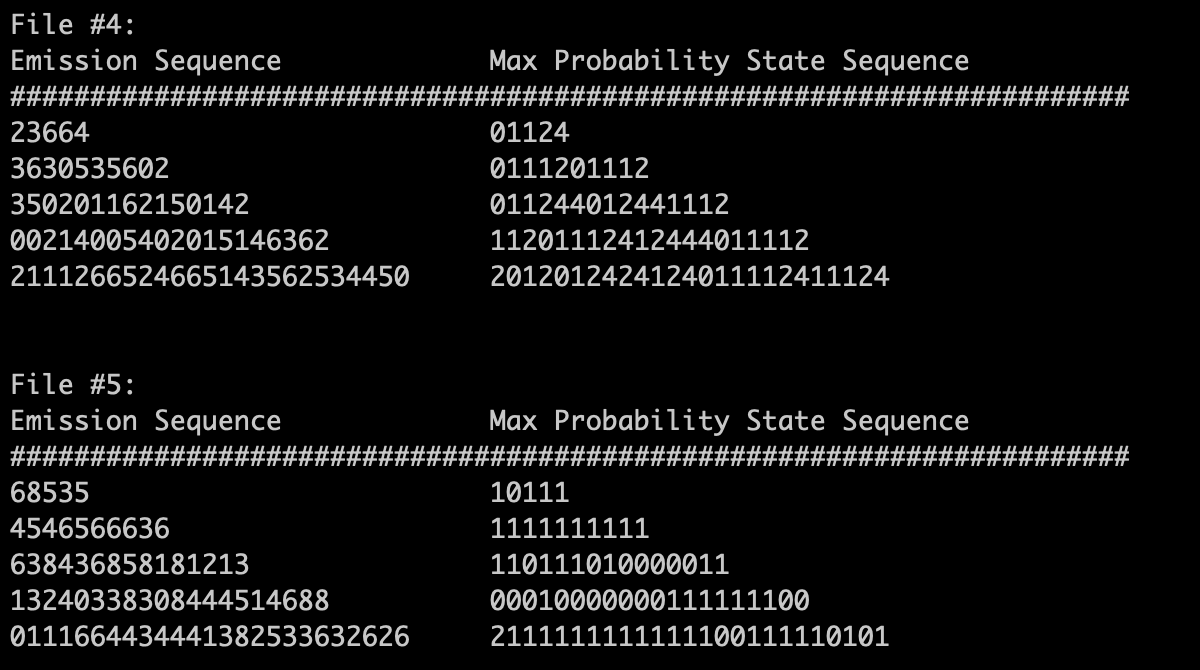
\includegraphics[width=0.5\textwidth]{img/set6template-f9aa7a5d.png}
  	\caption{}
  	\label{}
  \end{figure}
\end{subsolution}
\clearpage

\indent\problem[17] % indent for consistency
Probability of Emission Sequence for 6 Trained HMMs
\begin{subsolution}

Alphas on left, Betas on right

\begin{figure}[H]
	\centering
	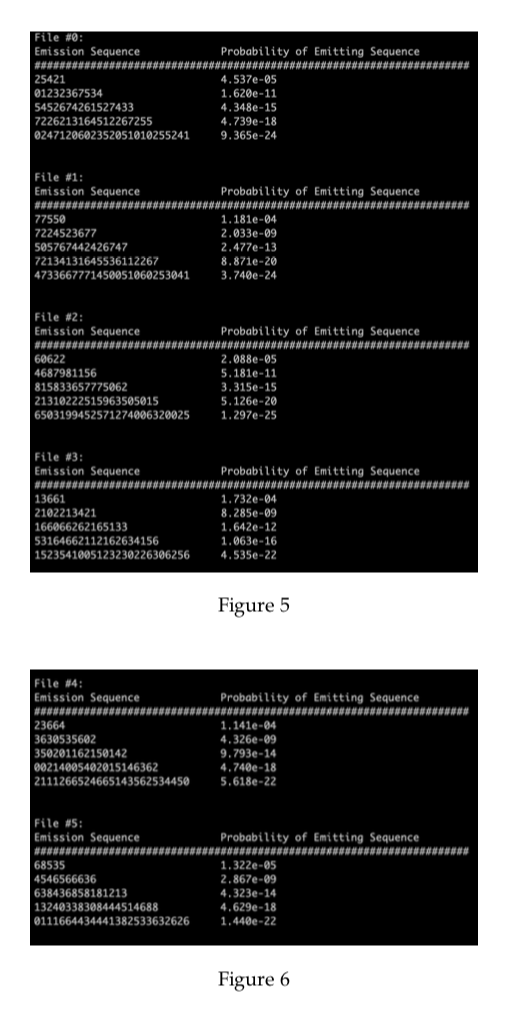
\includegraphics[width=0.49\textwidth]{img/set6template-18d875f7.png}
  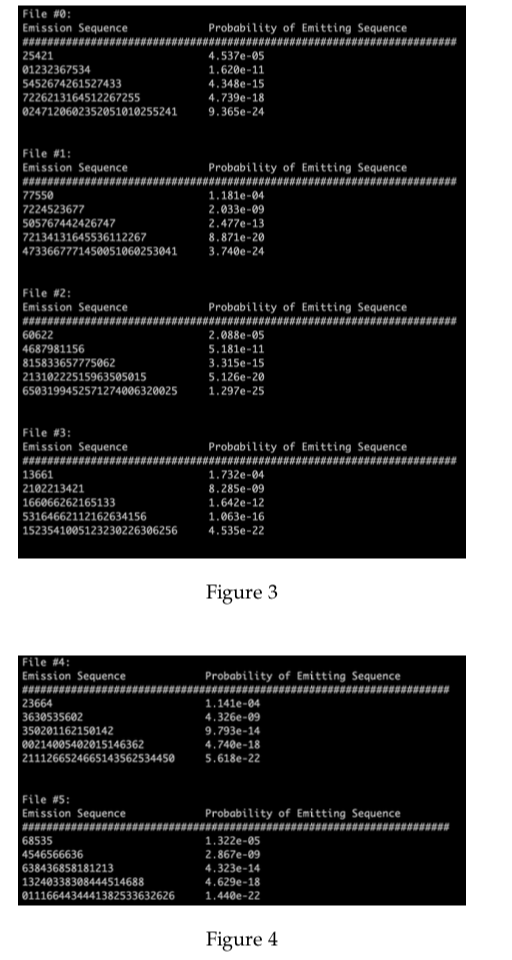
\includegraphics[width=0.49\textwidth]{img/set6template-438f3e5e.png}
	\caption{}
	\label{}
\end{figure}



\end{subsolution}
\clearpage

\noindent\problem[10] % indent for consistency
Learned State Transition and Output Emission Matrices of Supervised Hidden Markov Model
\begin{subsolution}
\begin{figure}[H]
	\centering
	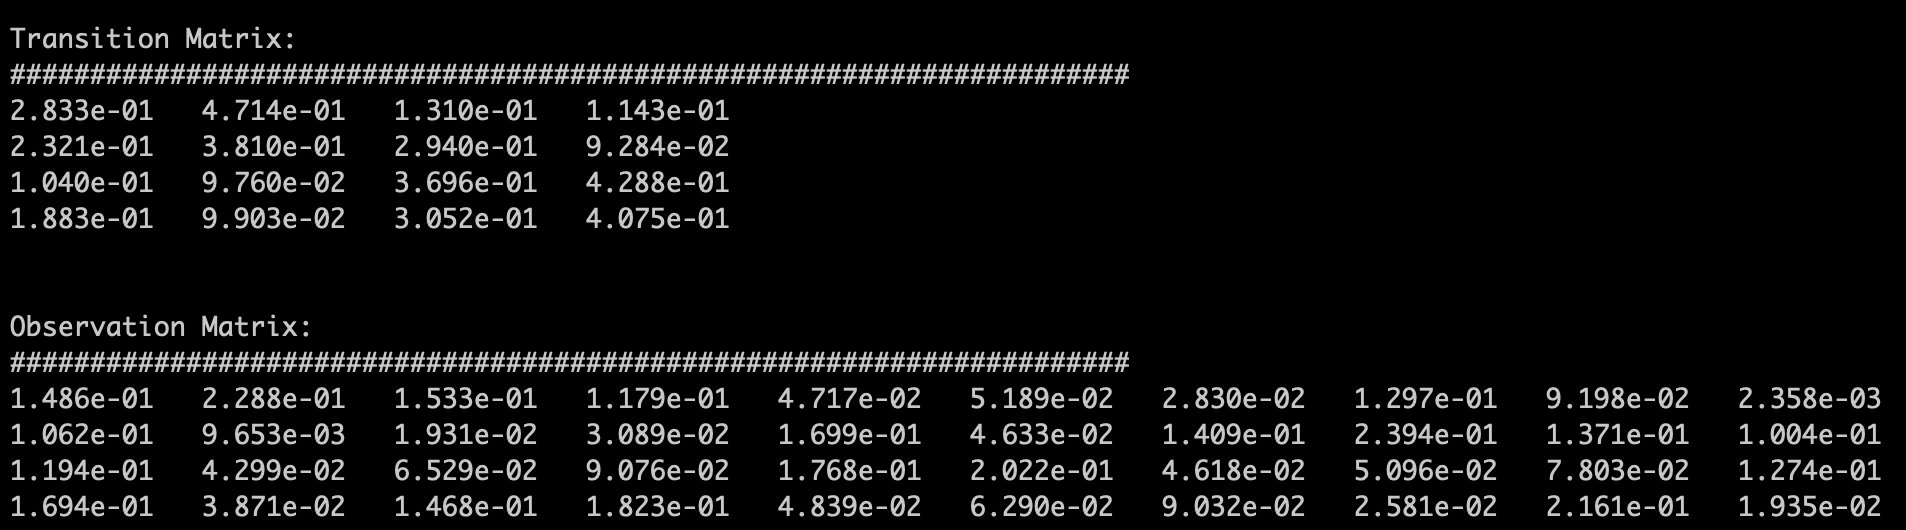
\includegraphics[width=0.5\textwidth]{img/set6template-70fa94d2.png}
	\caption{}
	\label{}
\end{figure}
\end{subsolution}
\clearpage

\indent\problem[15] % indent for consistency
Learned State Transition and Output Emission Matrices of Unsupervised Hidden Markov Model
\begin{subsolution}
\begin{figure}[H]
	\centering
	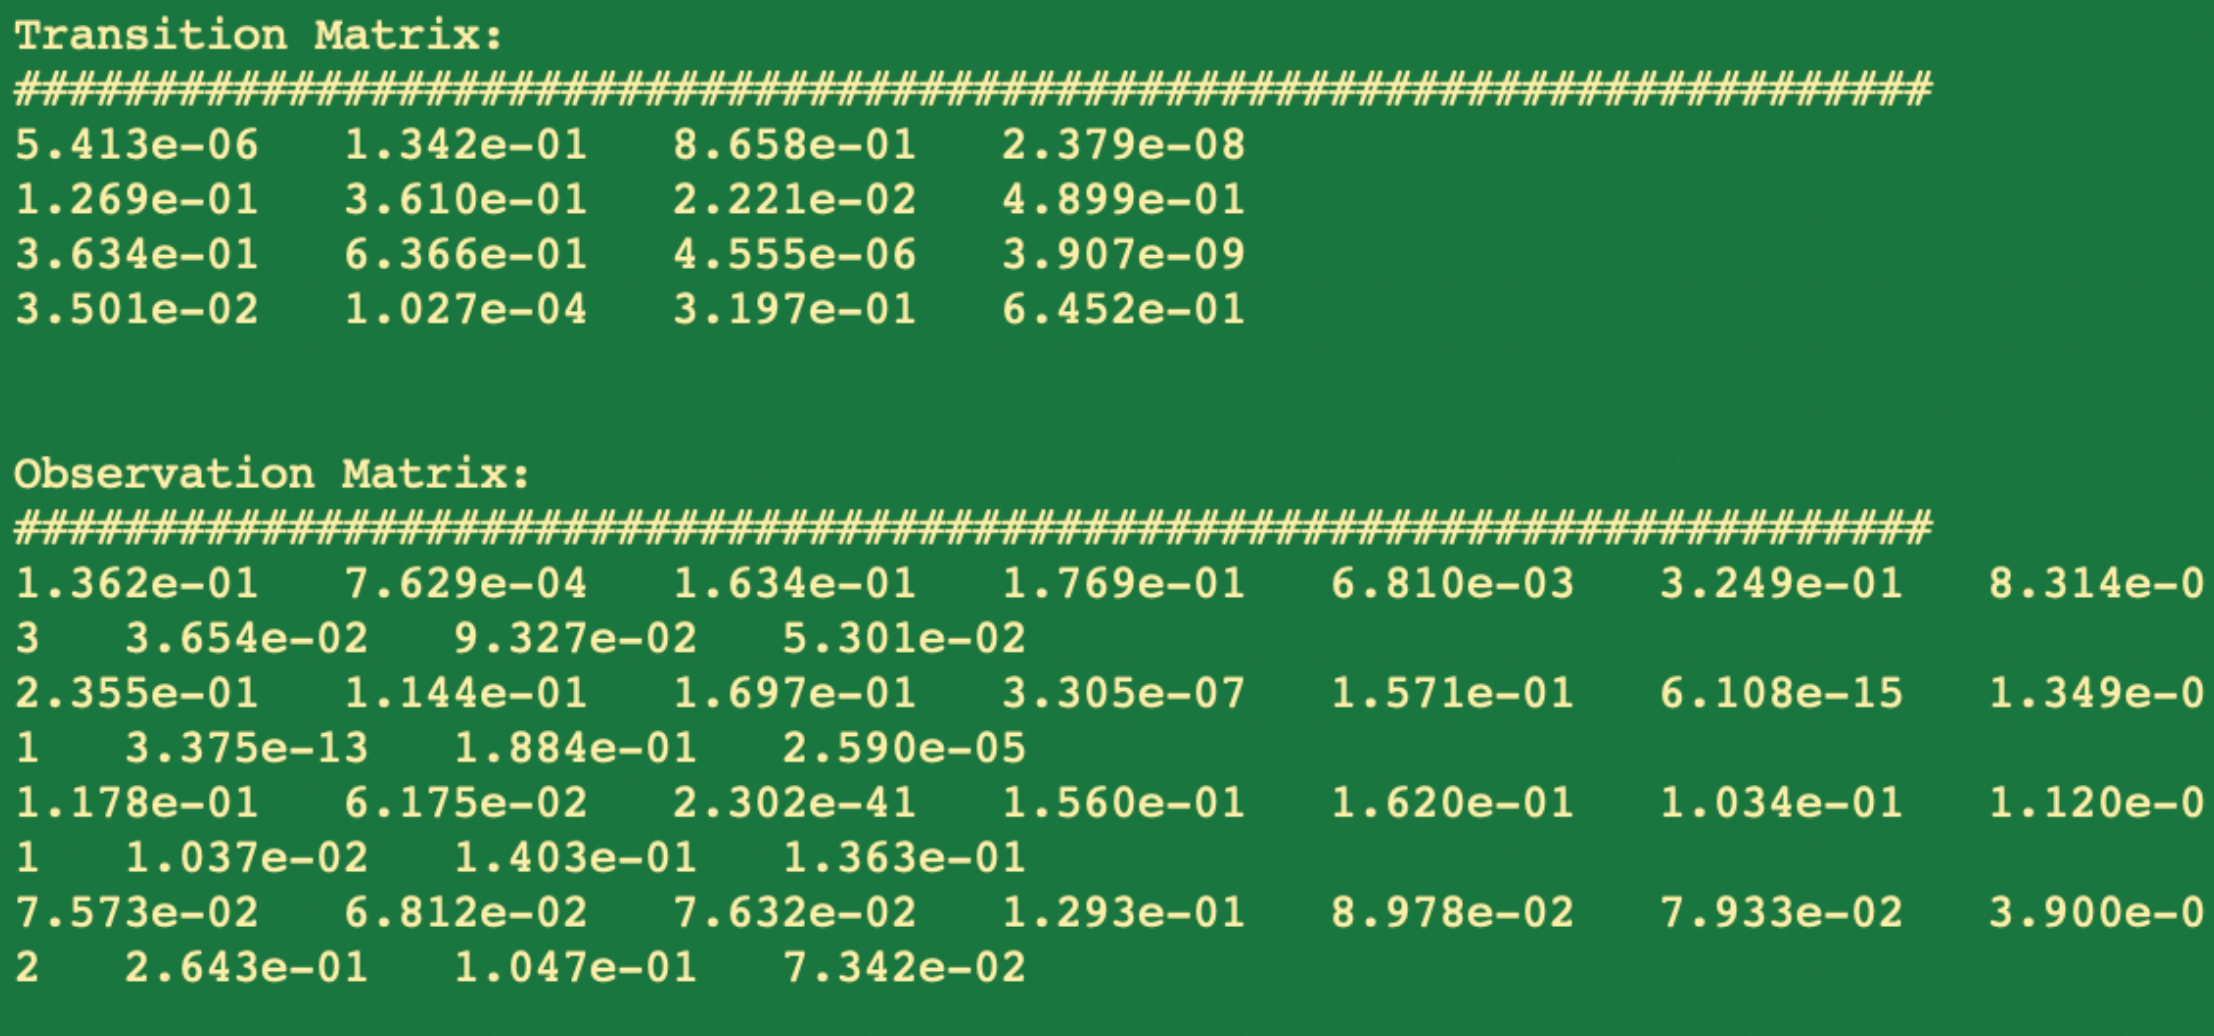
\includegraphics[width=0.5\textwidth]{img/set6template-ef31ef67.png}
	\caption{Note: this looks different because I ran it on my friend's computer because mine was performing very very slowly. I also
  seeded with 2019 (to check with Piazza). I know this seems fishy, but you can confirm the code in my submission, and I have unsupervised runs in the
  Jupyter notebook as well.}
	\label{}
\end{figure}
\end{subsolution}
\clearpage

\problem[5] Compare 2C and 2D
\begin{subsolution}
The variation in the unsupervised matrices is much more extreme; many values are either very close to 0 or decently close to 1 (in a geometric sense; many orders of magnitude larger than others).
The variation in the supervised matrices is less extreme.

Supervised offers a better approximation, as it involves training on observed state-emission pairings.

Unsupervised HMM's performance can be improved by training on additional data.



\end{subsolution}
\clearpage

\problem[5] Generating Emission Sequences
\begin{subsolution}
\begin{figure}[H]
	\centering
	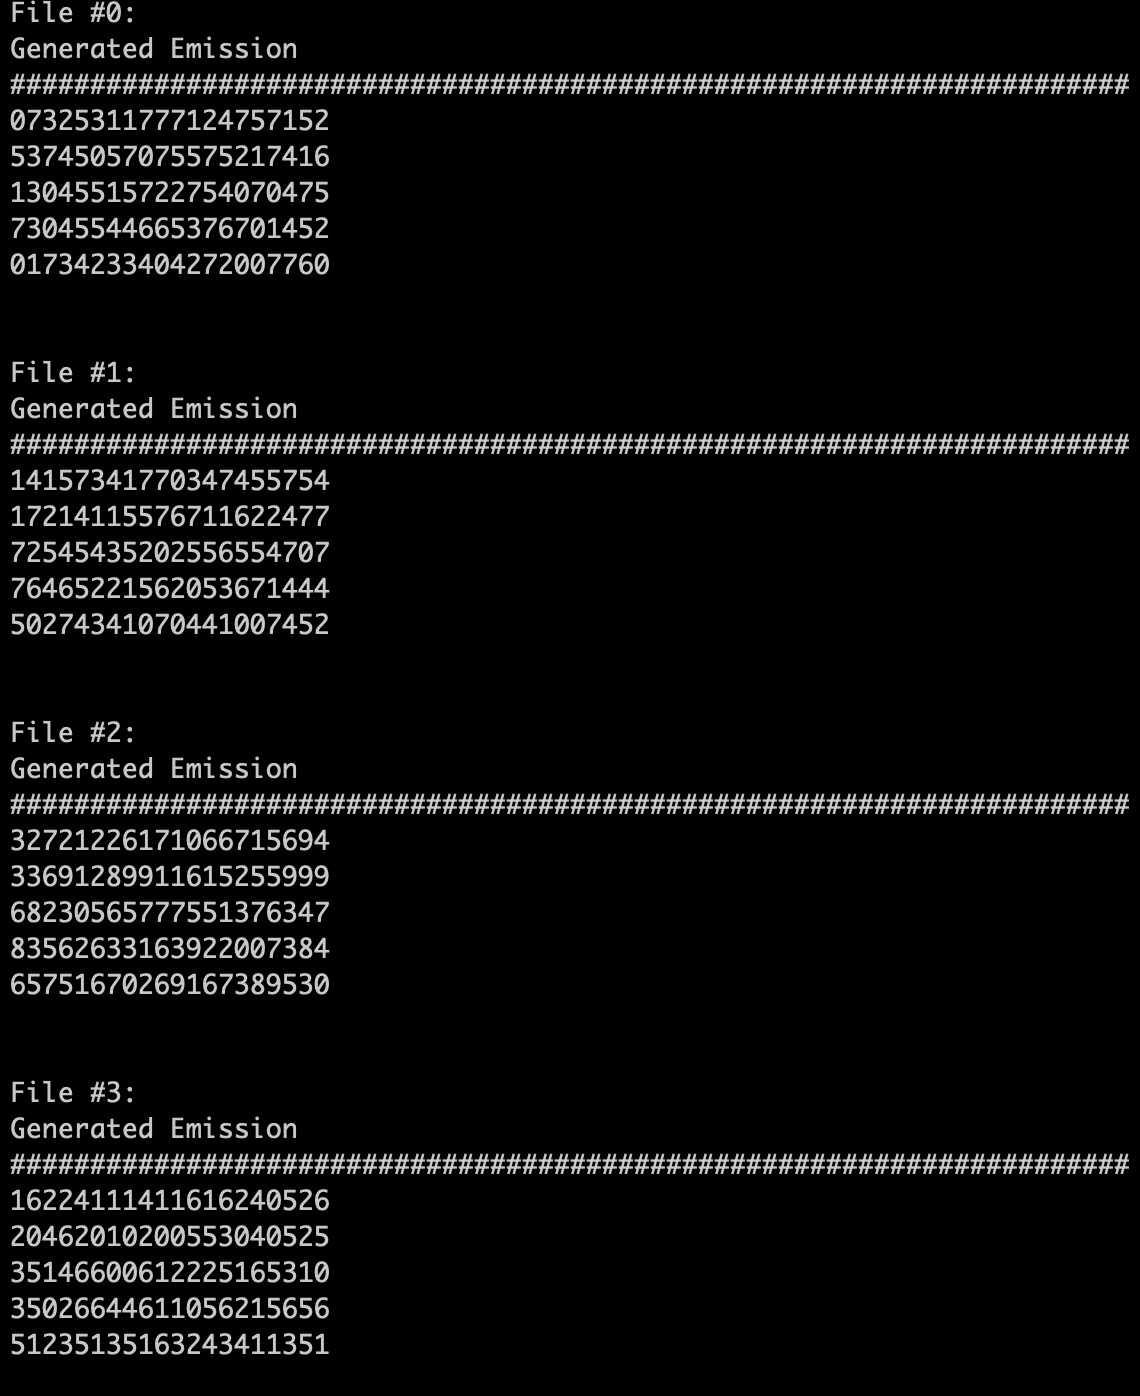
\includegraphics[width=0.5\textwidth]{img/set6template-4b947a80.png}
	\caption{}
	\label{}
\end{figure}
\begin{figure}[H]
	\centering
	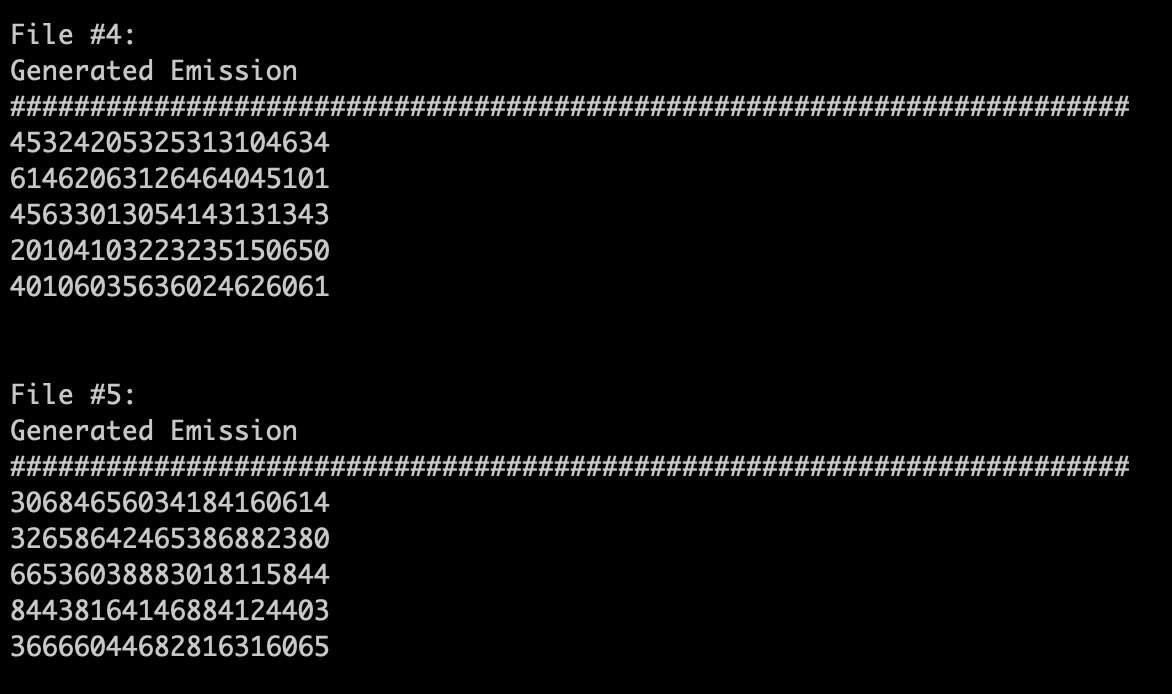
\includegraphics[width=0.5\textwidth]{img/set6template-c5d634e4.png}
	\caption{}
	\label{}
\end{figure}
\end{subsolution}
\clearpage

\indent\problem[3] % indent for consistency
Sparsity of Trained $A$ and $O$ Matrices
\begin{subsolution}
$A$ and $O$ seem mostly sparse; that is, each row/column has $0$ (or numbers very close to $0$) for the
majority of its entries.

This means that, from any state, there are realistically very few other states that are transitioned to, and very few emissions
that make sense in the context of this current state.
\end{subsolution}
\clearpage

\indent\problem[5] % indent for consistency
Hidden States vs. Sample Emission Sentences from HMM

\begin{subsolution}
In the case where there is one hidden state, the sentence is pretty nonsensical; it's simply a sequence of terms picked from the
frequency distribution of words in the document, as with only one state there's no distinguishing between the sampling distribution of
words in different positions.
As the number of hidden states increases, the sequences of words mirror more closely the kinds of sequences observed in the Constitution.
For example, in the most sophisticated model (16 hidden states), we have the phrase "regulate the united at importation declaring," which is pretty sequentially realistic.
In the less sophisticated models, the sentences are less and less sequentially logical.

In general, increasing the number of hidden states will increase the training data likelihood, because it will lead to fitting the training data more closely (and thus
mirroring its transitions more closely).
\end{subsolution}
\clearpage


\indent\problem[5] % indent for consistency
Analyzing Visualization of State
\begin{subsolution}
State 1 seems to have nouns - more specifically, nouns that represent significant entities in
the operation of a government; nouns like "senate," "congress," "state," "office," etc. While other states, like state 9, are also
composed primarily of nouns, they're more secondary in nature; state 9, for example, has nouns like "number," "resignation," "consequence," etc.
\end{subsolution}
\clearpage


\end{document}
